
\documentclass[11pt]{article}
\usepackage{amsmath,amssymb,geometry,booktabs,graphicx}
\usepackage{tikz}
\geometry{margin=1in}

\title{Five-State Estimation Model for a Differential Drive Robot}
\author{Dash Robot Miniature AV Stack -- Phase 1 (Open Loop Estimation)}
\date{}

\begin{document}
\maketitle

\section*{Overview}

This document defines a five–state kinematic model suitable for a miniature
autonomous vehicle (AV) estimation stack using a differential-drive robot.
Wheel encoder measurements are streamed to a host computer which runs an
Extended Kalman Filter (EKF) to estimate the robot state.

The estimator operates in discrete time with timestep $\Delta t$.

\section*{State Vector}

\begin{equation}
x_k =
\begin{bmatrix}
p_x \\
p_y \\
\theta \\
v \\
\omega
\end{bmatrix}
\in \mathbb{R}^{5}
\end{equation}

\begin{center}
\begin{tabular}{lll}
\toprule
State & Description & Units \\
\midrule
$p_x$ & Position in world $x$ direction & meters \\
$p_y$ & Position in world $y$ direction & meters \\
$\theta$ & Heading (yaw) angle & radians \\
$v$ & Forward velocity & m/s \\
$\omega$ & Yaw rate & rad/s \\
\bottomrule
\end{tabular}
\end{center}

\section*{Differential Drive Geometry}

\begin{center}
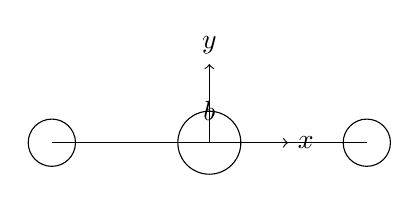
\begin{tikzpicture}[scale=1]
\draw (-2,0) circle (0.3);
\draw (2,0) circle (0.3);
\draw (-2,0)--(2,0);
\node at (0,0.4) {$b$};
\draw (0,0) circle (0.4);
\draw[->] (0,0)--(1,0) node[right] {$x$};
\draw[->] (0,0)--(0,1) node[above] {$y$};
\end{tikzpicture}
\end{center}

$b$ = distance between wheel contact points (meters).

\section*{Encoder Measurements}

Wheel encoders provide integer tick counts. Let

\begin{equation}
n_{L,k},\; n_{R,k}
\end{equation}

be cumulative tick counts at timestep $k$. The tick increments are

\begin{equation}
\Delta n_{L,k}=n_{L,k}-n_{L,k-1}
\end{equation}

\begin{equation}
\Delta n_{R,k}=n_{R,k}-n_{R,k-1}
\end{equation}

Wheel displacements are computed as

\begin{equation}
\Delta s_{L,k} = \frac{2\pi R}{N}\Delta n_{L,k}
\end{equation}

\begin{equation}
\Delta s_{R,k} = \frac{2\pi R}{N}\Delta n_{R,k}
\end{equation}

\begin{center}
\begin{tabular}{lll}
\toprule
Parameter & Description & Units \\
\midrule
$R$ & Wheel radius & meters \\
$N$ & Encoder ticks per revolution & ticks/rev \\
$b$ & Wheel baseline & meters \\
\bottomrule
\end{tabular}
\end{center}

\section*{Velocity Computation}

\begin{align}
v_{enc} &= \frac{\Delta s_R + \Delta s_L}{2\Delta t} \\
\omega_{enc} &= \frac{\Delta s_R - \Delta s_L}{b\Delta t}
\end{align}

Measurement vector

\begin{equation}
z_k =
\begin{bmatrix}
v_{enc} \\
\omega_{enc}
\end{bmatrix}
\in \mathbb{R}^{2}
\end{equation}

\section*{Process Dynamics}

\begin{align}
p_{x,k+1} &= p_{x,k} + v_k\cos(\theta_k)\Delta t \\
p_{y,k+1} &= p_{y,k} + v_k\sin(\theta_k)\Delta t \\
\theta_{k+1} &= \theta_k + \omega_k\Delta t \\
v_{k+1} &= v_k + w_v \\
\omega_{k+1} &= \omega_k + w_\omega
\end{align}

Compact form

\begin{equation}
x_{k+1} = f(x_k) + w_k
\end{equation}

\section*{Process Noise}

\begin{equation}
w_k =
\begin{bmatrix}
0 \\
0 \\
0 \\
w_v \\
w_\omega
\end{bmatrix}
\in \mathbb{R}^{5}
\end{equation}

\begin{equation}
w_k \sim \mathcal{N}(0,Q)
\end{equation}

\begin{equation}
Q \in \mathbb{R}^{5\times5}
\end{equation}

\section*{Measurement Model}

\begin{equation}
z_k = Hx_k + n_k
\end{equation}

\begin{equation}
H =
\begin{bmatrix}
0 &0 &0 &1 &0 \\
0 &0 &0 &0 &1
\end{bmatrix}
\in \mathbb{R}^{2\times5}
\end{equation}

\begin{equation}
n_k \sim \mathcal{N}(0,R), \quad R\in\mathbb{R}^{2\times2}
\end{equation}

\section*{EKF Prediction and Update}

Prediction:

\begin{align}
\hat{x}_{k|k-1} &= f(\hat{x}_{k-1|k-1}) \\
P_{k|k-1} &= F_kP_{k-1|k-1}F_k^T + Q
\end{align}

Update:

\begin{align}
K_k &= P_{k|k-1}H^T(H P_{k|k-1}H^T + R)^{-1} \\
\hat{x}_{k|k} &= \hat{x}_{k|k-1} + K_k(z_k - H\hat{x}_{k|k-1}) \\
P_{k|k} &= (I-K_kH)P_{k|k-1}
\end{align}

\section*{Jacobian of Process Model}

\begin{equation}
F_k =
\begin{bmatrix}
1 &0 &-v_k\sin\theta_k\Delta t &\cos\theta_k\Delta t &0 \\
0 &1 & v_k\cos\theta_k\Delta t &\sin\theta_k\Delta t &0 \\
0 &0 &1 &0 &\Delta t \\
0 &0 &0 &1 &0 \\
0 &0 &0 &0 &1
\end{bmatrix}
\in \mathbb{R}^{5\times5}
\end{equation}

\section*{Calibration of Robot Parameters}

Three parameters must be calibrated.

\subsection*{Wheel Radius $R$}

Drive the robot forward a known distance $D$ and record total encoder ticks $\Delta n$.

\begin{equation}
R = \frac{DN}{2\pi\Delta n}
\end{equation}

\subsection*{Ticks Per Revolution $N$}

Rotate a wheel manually and count encoder ticks for one full revolution.

\subsection*{Wheel Baseline $b$}

Command the robot to rotate in place $k$ full turns and record wheel travel.

\begin{equation}
b = \frac{\Delta s_R - \Delta s_L}{2\pi k}
\end{equation}

\section*{Block Diagram}

\begin{center}
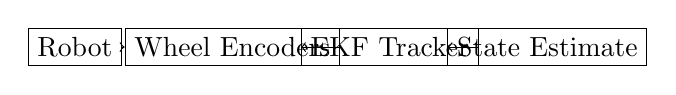
\begin{tikzpicture}[node distance=2cm]
\node (robot) [draw, rectangle] {Robot};
\node (enc) [draw, rectangle, right of=robot] {Wheel Encoders};
\node (host) [draw, rectangle, right of=enc] {EKF Tracker};
\node (state) [draw, rectangle, right of=host] {State Estimate};

\draw[->] (robot) -- (enc);
\draw[->] (enc) -- (host);
\draw[->] (host) -- (state);
\end{tikzpicture}
\end{center}

\end{document}
